\documentclass[tikz,border=6pt]{standalone}
\usetikzlibrary{arrows.meta}
\usepackage{amsmath, amssymb}

\begin{document}
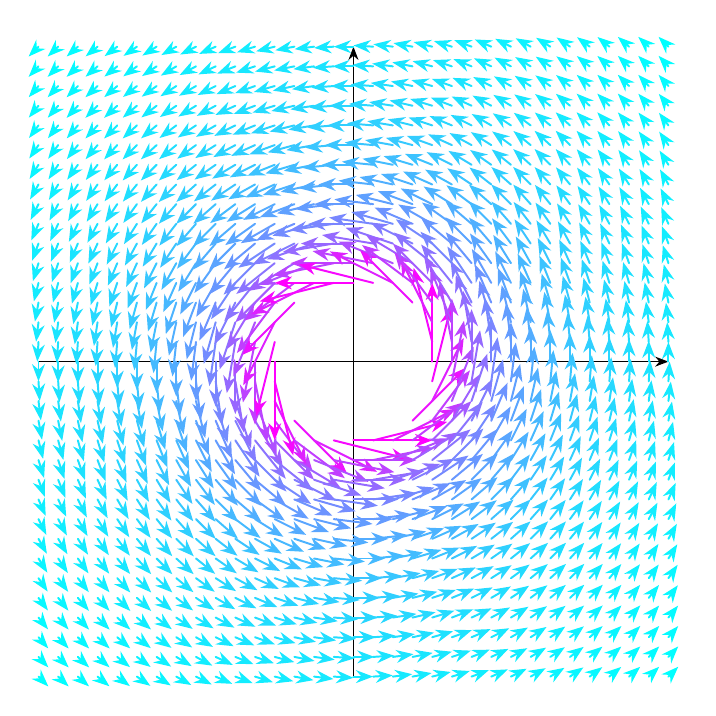
\begin{tikzpicture}[>=Stealth, line cap=round]
	% -------- Tunables --------
	\def\R{4}            % half-width of view (plots from -R..R)
	\def\step{0.25}       % grid spacing (arrow density)
	\def\arrowlen{1}   % arrow-length scale (true |F| ~ 1/r)
	
	% Axes (optional)
	\draw[thin,->] (-\R,0) -- (\R,0) node[below right] {};
	\draw[thin,->] (0,-\R) -- (0,\R) node[above left] {};
	
	% Visual cue: boundary of the excluded region x^2 + y^2 < 1
%		\draw[very thick, gray!60] (0,0) circle[radius=1];
	
	% Normalization for colormap (cool: cyan->magenta)
	% We'll map magnitude m = 1/sqrt(x^2+y^2) from [m_min, 1] to t in [0,1],
	% where m_min corresponds to the farthest grid corner (r ~ sqrt(2)*R).
	\pgfmathsetmacro{\mmin}{1/(sqrt(2)*\R)}  % lower bound of m over the square
	
	% Integer loop bounds
	\pgfmathtruncatemacro{\N}{\R/\step}
	
	% -------- Vector field on R^2 \ {(x,y): x^2+y^2 < 1} --------
	\foreach \i in {-\N,...,\N}{
		\foreach \j in {-\N,...,\N}{
			\pgfmathsetmacro{\X}{\i*\step}
			\pgfmathsetmacro{\Y}{\j*\step}
			\pgfmathsetmacro{\rsq}{\X*\X + \Y*\Y}  % r^2
			
			% Skip inside the unit disk
			\ifdim \dimexpr\rsq pt\relax < 1pt\relax
			% do nothing
			\else
			% Field components (scaled): F = (-y/(x^2+y^2), x/(x^2+y^2))
			\pgfmathsetmacro{\dx}{(-\Y/\rsq)*\arrowlen}
			\pgfmathsetmacro{\dy}{( \X/\rsq)*\arrowlen}
			
			% Magnitude and colormap parameter t in [0,1]
			\pgfmathsetmacro{\mag}{1/sqrt(\rsq)}                          % |F| = 1/r
			\pgfmathsetmacro{\tval}{(\mag - \mmin)/(1 - \mmin)}           % normalize
			\pgfmathsetmacro{\t}{min(1,max(0,\tval))}                     % clamp
			
			% "cool" colormap = linear from cyan (0,1,1) to magenta (1,0,1):
			%   R = t,  G = 1 - t,  B = 1
			\pgfmathsetmacro{\colR}{\t}
			\pgfmathsetmacro{\colG}{1-\t}
			\pgfmathsetmacro{\colB}{1}
			
			% ----- Draw the arrow (same API you wanted) -----
			\draw[->, line width=.25mm,
			draw={rgb,1:red,\colR; green,\colG; blue,\colB}]
			(\X,\Y) -- ++(\dx,\dy);
			\fi
		}
	}
%	\node[] at (8,0) {$\mathbf{F}(x,y)=\begin{bmatrix}
%			\displaystyle\frac{-y}{x^2+y^2}\\ \\ \displaystyle\frac{x}{x^2+y^2}
%		\end{bmatrix}\overset{\theta(x,y)=\arctan(y/x)}{=}\begin{bmatrix}
%		\displaystyle \frac{\partial}{\partial x}\theta\\ \\ \displaystyle\frac{x}{x^2+y^2}
%	\end{bmatrix}$};
	% (Optional) tiny legend: a short cool gradient bar
%	\foreach \k in {0,...,20}{
%		\pgfmathsetmacro{\t}{\k/20}
%		\pgfmathsetmacro{\colR}{\t}
%		\pgfmathsetmacro{\colG}{1-\t}
%		\pgfmathsetmacro{\colB}{1}
%		\fill[draw=none, fill={rgb,1:red,\colR; green,\colG; blue,\colB}]
%		(5.5,-5.7) ++(0.15*\k,0) rectangle ++(0.15,0.4);
%	}
%	\node[below] at (7,-5.7) {\small low $|\mathbf F|$ \hspace{1.5em} high};
	
\end{tikzpicture}
\end{document}


%\documentclass[tikz,border=6pt]{standalone}
%\usetikzlibrary{arrows.meta}
%
%\begin{document}
%\begin{tikzpicture}[>=Stealth, line cap=round]
%	% -------- Parameters you can tweak --------
%	\def\R{4}            % half-width of the view: plots from -R..R
%	\def\step{0.2}       % grid spacing (arrow density)
%	\def\arrowlen{1}   % global arrow length scale
%	
%	% Axes (optional)
%	\draw[thin,->] (-\R,0) -- (\R,0) node[below right] {$x$};
%	\draw[thin,->] (0,-\R) -- (0,\R) node[above left] {$y$};
%	
%	% Visual cue: unit circle boundary of the excluded region
%%		\draw[very thick, gray!60] (0,0) circle [radius=1];
%	
%	% Integer bounds for loops
%	\pgfmathtruncatemacro{\N}{\R/\step}
%	
%	% -------- Vector field on R^2 \ {(x,y): x^2+y^2 < 1} --------
%	\foreach \i in {-\N,...,\N}{
%		\foreach \j in {-\N,...,\N}{
%			\pgfmathsetmacro{\X}{\i*\step}
%			\pgfmathsetmacro{\Y}{\j*\step}
%			\pgfmathsetmacro{\rsq}{\X*\X + \Y*\Y} % r^2
%			
%			% Skip all points strictly inside the unit disk: x^2 + y^2 < 1
%			\ifdim \dimexpr\rsq pt\relax < 1pt\relax
%			% do nothing (excluded region)
%			\else
%			% F(x,y) = (-y/(x^2+y^2), x/(x^2+y^2)) scaled by \arrowlen
%			\pgfmathsetmacro{\dx}{(-\Y/\rsq)*\arrowlen}
%			\pgfmathsetmacro{\dy}{( \X/\rsq)*\arrowlen}
%			\draw[->, line width=.25mm, red] (\X,\Y) -- ++(\dx,\dy);
%			\fi
%		}
%	}
%\end{tikzpicture}
%\end{document}
